\subsection{Solving the DE}
We can solve these differential equation through separation of variables:

\textbf{Case 1: }
From 1 we have:

\begin{align*}
    -kv &= m \frac{dv}{dt}
    \\ \int \frac{1}{v} dv &= \int \frac{-k}{m} dt
    \\ \ln{(v)} &= \frac{-kt}{m} + c_1
    \\ v &= e^{\frac{-kt}{m} + c_1}
    \\ \Aboxed{v &= Ae^{\frac{-k}{m}t}}
\end{align*}

\textbf{Case 2:}
From 2 we have: 

\begin{align*}
    -kv - F_b &= m \frac{dv}{dt}
    \\ \int \frac{1}{-kv - F_b} dv &= \int \frac{1}{m} dt
    \\ -\frac{1}{k} \ln{(v + \frac{F_b}{k})} &= \frac{t}{m} + c_2
    \\ - \ln{(v + \frac{F_b}{k})} &= \frac{kt}{m} + c_2
    \\ v + \frac{F_b}{k} &= e^{-(\frac{kt}{m} + c_2)}
    \\ v &= e^{-(\frac{kt}{m} + c_2)} - \frac{F_b}{k}
    \\ \Aboxed{v &= Ae^{-(\frac{k}{m}t)} - \frac{F_b}{k}}
\end{align*}

\subsection{Solutions of the DE}
\textbf{Case1: } 
Using the initial conditions, we can find v as a function of t
\\ \\
Using the point (t=0, v=96), we see that:
\begin{center}
\begin{align*}
    v &= Ae^{\frac{-kt}{m}}
    \\ 96 &= Ae^0
    \\ A &= 96
\end{align*}
\end{center}
Using the point (t=9, v=55), we see that:
\begin{center}
\begin{align*}
    v &= Ae^{\frac{-kt}{m}}
    \\ 55 &= 96e^{\frac{-kt}{m}}
    \\ \frac{55}{96} &= e^{(\frac{-9k}{m})}
    \\ \ln{(\frac{55}{96})} &= \frac{-9k}{m}
    \\ k &= -\frac{1}{9}m\ln{(\frac{55}{96})}
    \\ &= \text{7426.87 $N/ms^{-1}$}
\end{align*}
\end{center}

Using the result $k=\frac{k}{m} = 0.0619$ From this we can deduce that for case 1:
\begin{equation}
    \boxed{v = 96e^{-0.0619}}
\end{equation}

\textbf{Case 2: } 
Using the initial conditions, we can find v as a function of t
\\ \\
Using the point (t=9, v=55), we see that:
\begin{align*}
    v &= Ae^{-(\frac{kt}{m})} - \frac{F_b}{k}
    \\ 55 &= Ae^{-(\frac{9k}{m})} - \frac{F_b}{k}
\end{align*}
\\
Using the point (t=26, v=0), we see that:

\begin{center}
\begin{align*}
    v &= Ae^{-(\frac{kt}{m})} - \frac{F_b}{k}
    \\ 0 &= Ae^{-(\frac{26k}{m})} - \frac{F_b}{k}
\end{align*}
\end{center}

Therefore by solving the simultaneous equation we find:
\begin{align*}
    A &= \frac{40847963}{276821}
    \\ &= 147.56
    \\ F_b &= \frac{6069149494577}{27682100}
    \\ &= 219244.5
\end{align*}
Therefore we can conclude that for case 2:
\begin{equation}
    \boxed{v = 147.56e^{(-0.0619x)} - 29.5}
\end{equation}

\subsection{Model Performance}

\begin{table}[H]
\centering
    \begin{tabular}{|l|l|l|l|l|l|l|l|l|l|l|l|l|l|l|l|l|}
        \hline
        t(s) & 0 & 1 & 2 & 3 & 4 & 5 & 6 & 7 & 8 & 9 \\ \cline{1-11} 
        predicted v(m/s) & 96.00 & 90.24 & 84.82 & 79.73 & 74.95 & 70.45 & 66.22 & 62.25 & 58.51 & 55.00
        \\ \cline{1-11}
        Actual v(m/s) & 96 & 89 & 82 & 77 & 72 & 68 & 64 & 61 & 58 & 55 \\ \cline{1-11}
        $d^2$ & 0.000 & 1.534 & 7.970 & 7.467 & 8.688 & 6.001 & 4.936 & 1.556 & 0.262 & 0.000 \\ \cline{1-11}
    \end{tabular}
    \caption{Case 1}
    \vspace{0.5cm}

    \begin{tabular}{|l|l|l|l|l|l|l|l|l|l|l|l|}
        \hline
        t(s) & 10 & 11 & 12 & 13 & 14 & 15 & 16 & 17 & 18 \\ \cline{1-10}
        predicted v(m/s) & 49.95 & 45.18 & 40.69 & 36.48 & 32.52 & 28.80 & 25.30 & 22.01 & 18.91 \\ \cline{1-10}
        Actual v(m/s) & 50 & 46 & 41 & 38 & 34 & 31 & 27 & 24 & 21 \\ \cline{1-10}
        $d^2$ & 0.003 & 0.677 & 0.093 & 2.308 & 2.191 & 4.855 & 2.901 & 3.972 & 4.349 \\ \cline{1-10}
    \end{tabular}
    \caption{Case 2}
    \vspace{0.5cm}

    \begin{tabular}{|l|l|l|l|l|l|l|l|l|}
        \hline
        t(s) & 19 & 20 & 21 & 22 & 23 & 24 & 25 & 26 \\ \cline{1-9}
        predicted v(m/s) & 16.01 & 13.28 & 10.71 & 8.29 & 6.02 & 3.89 & 1.89 & 0.00 \\ \cline{1-9}
        Actual v(m/s) & 18 & 16 & 13 & 10 & 8 & 5 & 3 & 0
        \\ \cline{1-9}
        $d^2$ & 3.969 & 7.422 & 5.257 & 2.914 & 3.905 & 1.231 & 1.242 & 0.000 \\ \cline{1-9}
    \end{tabular}
    \caption{Case 2 continued}
\end{table}

\begin{figure}[H]
\centering

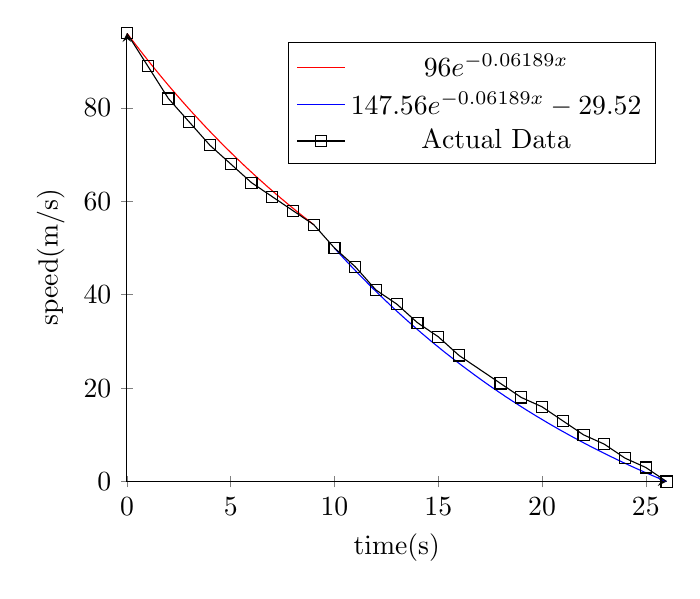
\begin{tikzpicture}
\begin{axis}[
    axis lines = left,
    xlabel = time(s),
    ylabel = speed(m/s),
]
%Below the red parabola is defined
\addplot [
    domain=0:9,
    samples=100, 
    color=red,
]
{96*e^(-0.06189*x)};
\addlegendentry{$96e^{-0.06189x}$}
%Here the blue parabloa is defined
\addplot [
    domain=10:26, 
    samples=100, 
    color=blue,
    ]
    {147.56*e^(-0.06189*x) - 29.52};
\addlegendentry{$147.56e^{-0.06189x}-29.52$}
 
 \addplot[
    color=black,
    mark=square]
    coordinates {(0,96)(1,89)(2,82)(3,77)(4,72)(5,68)(6,64)(7,61)(8,58)(9,55)(10,50)(11,46)(12,41)(13,38)(14,34)(15,31)(16,27)(18,21)(19,18)(20,16)(21,13)(22,10)(23,8)(24,5)(25,3)(26,0)};
\addlegendentry{Actual Data}
\end{axis}
\end{tikzpicture}
\caption{Graph showing the predicted velocity values against the actual velocity values}
\end{figure}